%!TEX root = ../index.tex
Im Kapitel~\ref{cha:fehlerkatalog} sind insgesamt 36 Fehlerszenarios Katalogisiert. Um Lösungen für diese Szenarios zu finden, wurden diese zuerst in verschiedene Gruppen eingeteilt.

\section{Nicht automatisiert testbare Fehlerszenarios}
\label{sec:nicht_automatisiert_testbare_fehlerszenarios}
Einige Fehlerszenarios sind nicht oder nur mit unverhältnismässigem Aufwand automatisiert testbar.

\ref{f:missverhalten}, \ref{f:fourofourhandling}, \ref{f:seitefunktioniertnichtaufmobilengeraeten}, \ref{f:rechtschreibefehler}, \ref{f:falschaufbereitetebilder}, \ref{f:designverletzt}, \ref{f:fehlmanipulationdurchdenkunden}, \ref{f:deeplinksfunktionierennicht}

\section{Teilautomatisiert testbare Fehlerszenarios}
\label{sec:teilautomatisiert_testbare_fehlerszenarios}
Zwei Fehlerszenarios können nicht komplett automatisiert werden, sie können jedoch zu einem hohen Grad durch ein System unterstützt werden.

\subsubsection{Abhängigkeiten mit Sicherheitslücken}
\label{ssub:kat_abhaengigkeitenmitsicherheitsluecken}
\ref{f:abhaengigkeitenmitsicherheitsluecken} kann insofern automatisiert werden, dass ein Entwickler, welcher über die Mailingliste der entsprechenden Abhängigkeit von einer Sicherheitslücke erfährt, ein System verwendet welches ihm eine Auswertung der verwendeten Versionen dieser Abhängigkeit über alle laufenden Projekte ermöglicht.

\subsubsection{Browser spezifische Probleme}
\label{ssub:kat_browser_spezifische_probleme}
\ref{f:browserspezifischeprobleme} Da es zu viele verschiedene Browser gibt um eine Webprojekt mit allen zu Testen, wird meist mit den Browsern getestet, welche den höchsten Anteil an Besuchen haben. Um Fehler welche durch neuere Browser entstehen zu bemerken, kann jedoch ein ``\acrlong{rum}'' \glsadd{real_user_monitoring} verwendet werden. Damit wird das Verhalten des Benutzers direkt aufgezeichnet. Falls nun ein Problem mit einem spezifischen Browser besteht, werden verschiedene Kennzahlen für diesen Browser von den Normalwerten abweichen. Durch ein geschicktes setzen von Toleranzwerden und Benachrichtigungen, können so die gröbsten Probleme erfasst werden.

\section{Fehlerszenarios welche bereits abgedeckt werden}
\label{sec:fehlerszenarios_welche_bereits_abgedeckt_werden}
Die im Abschnitt~\ref{sec:eingesetzte_mittel_für_die_qualitätssicherung} beschriebenen Mittel decken bereits einige Fehlerszenarios ab. Diese Fehlerszenarios müssen nicht von den zu evaluierenen Systemen abgedeckt werden. Jedoch kann es sein, dass nach dieser Arbeit einige Fehlerszenarios mehrfach abgedeckt sind, was dazu führen kann, dass in den Mitteln aus Abschnitt~\ref{sec:eingesetzte_mittel_für_die_qualitätssicherung} diese Szenarios nicht mehr abgedeckt werden müssten. Abbildung~\ref{fig:uebersicht_fehlerszenarios} zeigt welche Fehlerszenarios bereits abgedeckt und welche noch offen sind.

\begin{table}[h!]
  \centering
  \begin{tabular}{lll}
  \toprule
    Nummer & Bezeichnung & Abgedeckte Fehler\\
  \hline
    \ref{b:precommithook} & Precommit Hook & \ref{f:codeconventions}, \ref{f:syntaxfehler}\\
  \hline
    \ref{b:sentry} & Sentry & \ref{f:cronjobfehler}, \ref{f:workerfehler}, \ref{f:fehlerimproduktivsystem}, \ref{f:javascriptfehler}\\
  \hline
    \ref{b:golivecheckliste} & Go-Live Checkliste & \ref{f:fourofourhandling}, \ref{f:seitefunktioniertnichtaufmobilengeraeten}, \ref{f:ogtagsfehlerhaftodernichtvorhanden}, \ref{f:metadescriptionundseitentitel}, \ref{f:deeplinksfunktionierennicht} \\
  \hline
    \ref{b:deploymentprozess} & Deployment-Prozess & \ref{f:cssfehler}\\
  \bottomrule
  \end{tabular}
  \caption{Abdeckung von Fehlerszenarios durch bestehende Massnahmen}
  \label{tab:abdeckung_von_fehlerszenarios_durch_bestehende_massnahmen}
\end{table}

\begin{figure}[h]
\centering
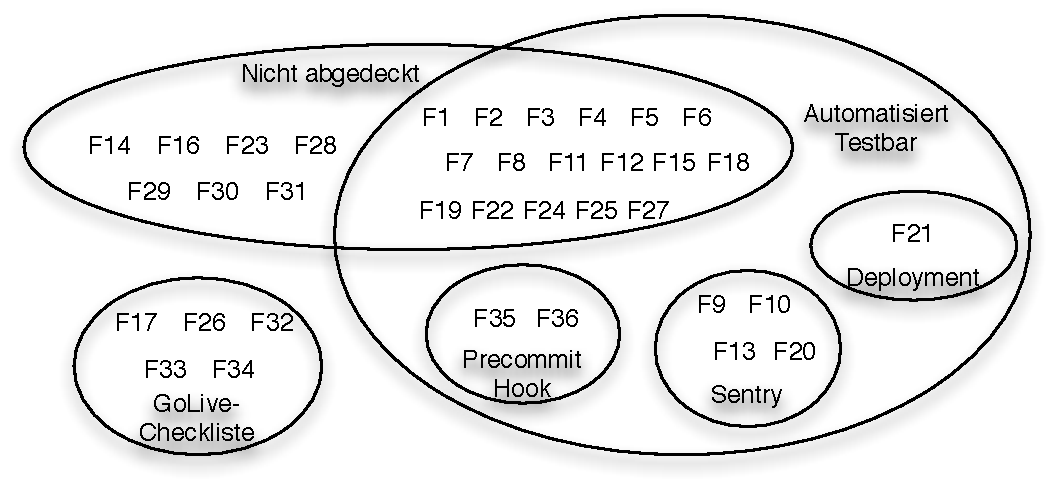
\includegraphics[width=1\textwidth]{images/abdeckung.pdf}
\caption{Übersicht Fehlerszenarios}
\label{fig:uebersicht_fehlerszenarios}
\end{figure}

\section{Fehlerszenarios welche abgedeckt werden müssen}
\label{sec:fehlerszenarios_welche_abgedeckt_werden_müssen}
Die Fehlerszenarios welche nicht durch die bereits vorhandenen Systeme abgedeckt werden, sollen gemäss Aufgabenstellung in automatisiert und manuell testbar unterteilt werden. Als manuell testbar ist ein Szenario dann, wenn es durch eine Software geprüft werden kann. So sind zum Beispiel Rechtschreibfehler nicht automatisiert prüfbar, da zur Zeit keine Rechtschreibprüfung vollautomatisiert arbeiten kann. Es ist immer zusätzlich ein Mensch nötig welcher entscheiden muss, ob zum Beispiel ein Wort ein Name ist und daher nicht im Wörterbuch zu finden ist.

\subsubsection{Automatisiert testbar}
\label{ssub:automatisiert_testbar}

\ref{f:zertifikatausgelaufen} \fzertifikatausgelaufen, \ref{f:zertifikatungultig} \fzertifikatungultig, \ref{f:sslnichterzwungen} \fsslnichterzwungen, \ref{f:externeassetsohnessl} \fexterneassetsohnessl, \ref{f:domainausgelaufen} \fdomainausgelaufen, \ref{f:dnsservernichtverfuegbar} \fdnsservernichtverfuegbar, \ref{f:dnseintragfehlerhaft} \fdnseintragfehlerhaft, \ref{f:spfeintragfehlerhaft} \fspfeintragfehlerhaft, \ref{f:deprecatedlibraries} \fdeprecatedlibraries, \ref{f:unittestfehler} \funittestfehler, \ref{f:debugmodus} \fdebugmodus, \ref{f:datenbankquerieslaufenlangsam} \fdatenbankquerieslaufenlangsam, \ref{f:applikationlaeuftlangsam} \fapplikationlaeuftlangsam, \ref{f:seitelaedtzulangsam} \fseitelaedtzulangsam, \ref{f:assetsfehlen} \fassetsfehlen, \ref{f:externeabhaengigkeiten} \fassetsfehlen, \ref{f:seiteenthaelttotelinks} \fseiteenthaelttotelinks

\subsubsection{Manuell testbar}
\label{ssub:manuel_testbar}

\ref{f:missverhalten} \fmissverhalten, \ref{f:abhaengigkeitenmitsicherheitsluecken} \fabhaengigkeitenmitsicherheitsluecken, \ref{f:browserspezifischeprobleme} \fbrowserspezifischeprobleme, \ref{f:rechtschreibefehler} \frechtschreibefehler, \ref{f:falschaufbereitetebilder} \ffalschaufbereitetebilder, \ref{f:designverletzt} \fdesignverletzt, \ref{f:fehlmanipulationdurchdenkunden} \ffehlmanipulationdurchdenkunden
